\chapter{Instructions}
\label{chap:instructions}

The following table shows some of the most important packages\index{packages} used in the \LaTeX{} template.

\begin{table}[H]
	\centering
		\begin{tabular}{p{0.13\textwidth} p{0.75\textwidth}} \toprule
			\textbf{Package} & \textbf{Function} \\ \midrule
			\texttt{cmbright}\index{cmbright} & sans serif font "Computer Modern Bright", which supports text encodings\index{text encodings} OT1, T1 and TS1, as well as the mathematical signs and AMS symbols \\ \midrule
			\texttt{ae} & provides better resolution fonts in PDF files \\ \midrule
			\texttt{fancyhdr}\index{fancyhdr} & easy adjustment of head- and foot lines \\ \midrule
			\texttt{graphicx}\index{graphicx} & integration of graphics in \LaTeX{} documents \\ \midrule
			\texttt{booktabs}\index{booktabs} & better presentation of tables \\ \midrule
			\texttt{textpos}\index{textpos} & simplified and absolute positioning of boxes on the page \\ \midrule
			\texttt{hyperref}\index{hyperref} & package to complie links into PDF files \\ \midrule
			\texttt{geometry}\index{geometry} & simplified and improved adaptation of the standard type area \\ \midrule
			\texttt{makeidx}\index{makeidx} & simple Index compilation (see section \ref{sec:instructions_index}) \\ \midrule
			\texttt{glossaries}\index{glossaries} & compilation of glossaries (see section \ref{sec:instructions_glossay}) \\ \bottomrule
		\end{tabular}
	\caption{Packages}
	\label{tab:packages}
\end{table}


\section{Subject Indices}
\label{sec:instructions_index}

\LaTeX{} is not able to create an \gls{Index}\index{Index} in the basic configuration. This can be created in \LaTeX{} with the \texttt{makeidx} package and the \texttt{makeindex}\index{makeindex} program. The following page contains a detailed explanation of how the package works, and its application:

\begin{center}
	\url{http://en.wikibooks.org/wiki/LaTeX/Indexing}
\end{center}

Roughly summarized the following points are needed for an index:

\begin{itemize}
	\item Embed the package \texttt{makeidx}.
	\item Initialize the compilation with the command \texttt{\textbackslash makeindex}.
	\item Continuously initializing words in the text with the command \texttt{\textbackslash index\{\}}.
	\item During the first passage of the document's compilation, the directory is created and definitions marked with \texttt{\textbackslash index\{\}} are stored in the \texttt{.idx} file.
	\item During the second passage the \texttt{.idx} file is sorted, formatted and stored as \texttt{.ind} file whereas \LaTeX{} then inserts the \texttt{.ind} file into the document.
\end{itemize}

\section{Glossay}
\label{sec:instructions_glossay}

A glossary\index{glossary} can also be created in \LaTeX{} with the \texttt{makeindex} program and the \texttt{glossaries} package. The following list shows the procedure to generate a glossary:

\begin{itemize}
	\item Integration of the package \texttt{glossaries}.
	\item If necessary, a personal database may be created including glossary entries. This template works with such a database, which is stored in the \texttt{database}folder. Entries from the database are only written in the directory if the word in the text is actually stated.
	\item With the \texttt{\textbackslash makeglossaries} command a new compilation is initialized.
	\item New entries can be created with the command \\ \texttt{\textbackslash newglossaryentry\{<SHORTCUT>\}\{name=\{<NAME>\},description=\{<DESCRIPTION>\}\}}.
	\item In the text continuously referencing words with the command \texttt{\textbackslash gls\{<SHORTCUT>\}}.
	\item Similar to the compilation of the index, the directory is only embedded into the document  during the second passage.
\end{itemize}

In order to work accurately, the glossary must be compiled with \texttt{makeindex} after post-editing the document. For this the following code in the command line is to be executed:

\begin{center}
	\texttt{makeindex -s template.ist -t template.glg -o template.gls template.glo}
\end{center}

With most \LaTeX editors, this can be stated as a post-processing step. The following explanation is for the TeXnicCenter program. Under the menu "Build" > "Define Output Profile..." (short: alt + F7) in the "Postprocessor" register, the window shown in Figure \ref{fig:postprocessing} can be found. Then it is necessary to insert a new entry, when an application as well as an argument must be specified. The application can be found in the MiKTeX installation (\texttt{..\textbackslash MiKTeX X.X\textbackslash miktex\textbackslash bin\textbackslash makeindex.exe}). As an argument, the following line must be entered:

\begin{center}
	\texttt{-s \string"\%tm.ist\string" -t \string"\%tm.glg\string" -o \string"\%tm.gls\string" \string"\%tm.glo\string" }
\end{center}

\begin{figure}[H]
	\centering
		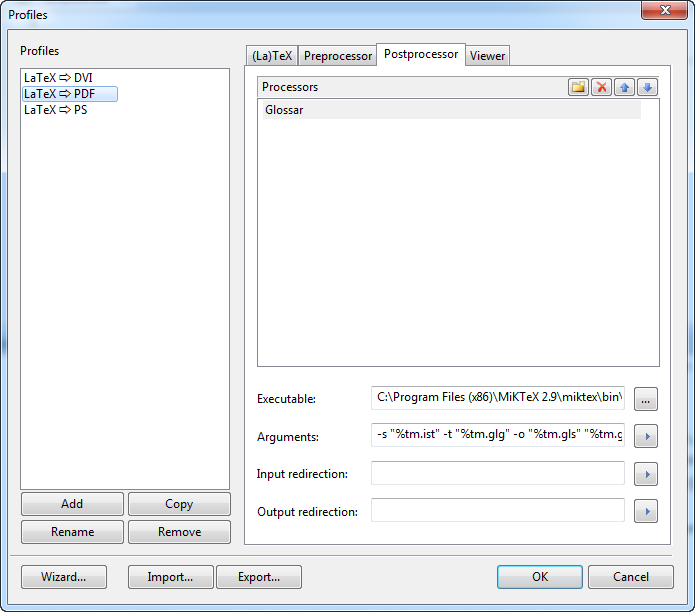
\includegraphics[scale=0.6]{images/profiles_glossar.png}
	\caption{Post-processing}
	\label{fig:postprocessing}
\end{figure}


\section{Bibliography}
\label{sec:instructions_bibliography}

To compile a bibliography\index{bibliography} one must resort to \gls{BibTeX}. The folder \texttt{database} includes a \texttt{.bib} file with various database entries. How the entries are to be compiled, can be taken from various sources of the Internet or books. The entries in the database will only be written to the directory of the document when the source is actually cited in the text.

Under the following addresses further explanations are found in order to compile the database and its use:

\begin{itemize}
	\item \url{http://en.wikipedia.org/wiki/BibTeX}
	\item \url{http://www.bibtex.org/}
\end{itemize}


